\section{Component View}
L'applicazione presente sul server \textit{LVSEmergency} è una \textit{Spring Boot Application} tramite cui vengono gestite le richieste HTTP/REST inviate dalla \textit{Client Application}.
Per l'implementazione dei microservizi REST è stato utilizzato un modello esagonale: ogni componente all'interno del server \textit{LVSEmergency} sarà costituito da un \textit{REST Controller}, un'\textit{ApplicationService} e agirà sul \textit{Domain Model}. In questo modo, ogni servizio è implementato in modo autonomo e non c'è interazione tra loro.
\todo{da rileggere}
\begin{figure}[h!]
	\centering
	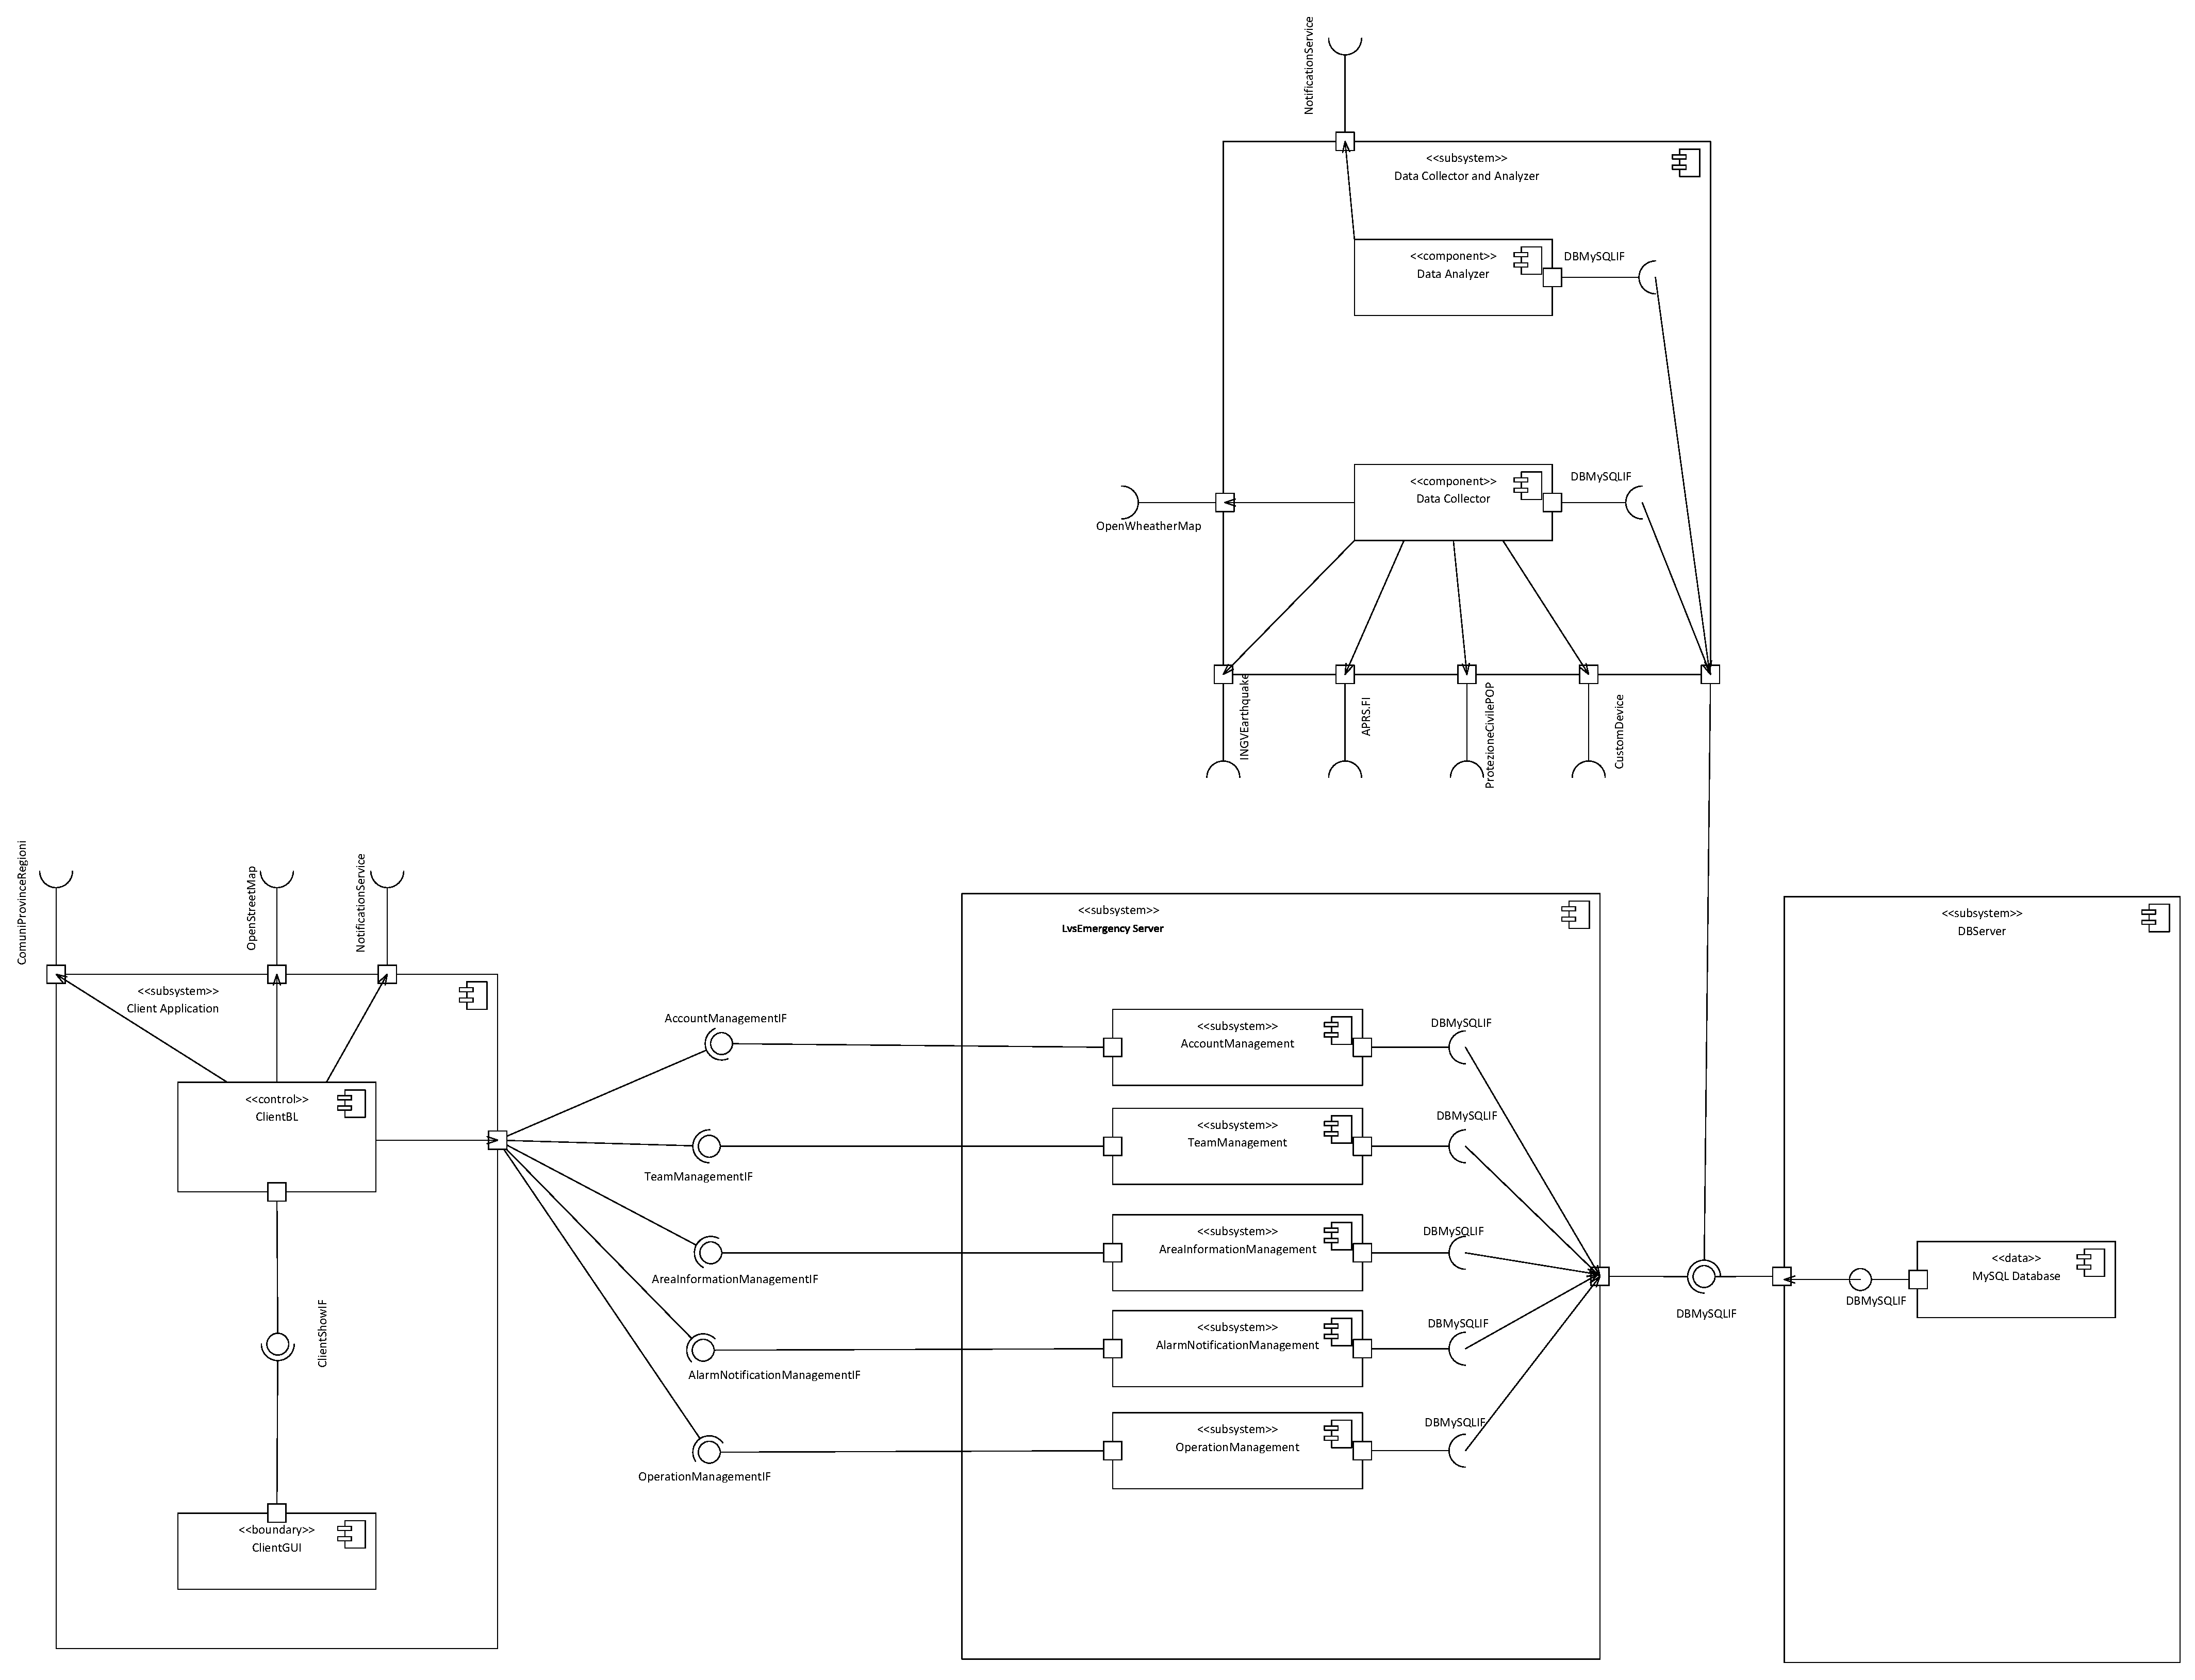
\includegraphics[width=1\linewidth]{./Iterazione 1/OtherFiles/UML - Component View}
	\caption{Component Diagram.}
	\label{fig:ComponentDiagram}
\end{figure}